\documentclass[12pt, a4paper]{article}

\usepackage[utf8]{inputenc}
\usepackage[ngerman]{babel}
\usepackage[T1]{fontenc}
\usepackage{graphicx}
\usepackage{pifont}% http://ctan.org/pkg/pifont

\title{Lastenheft}

\begin{document}

\maketitle
\pagebreak
\tableofcontents
\pagebreak

\section{Zielbestimmung}

Im Dezember 2019 erteilte der Lehrstuhl für Softwaretechnologie der TU Dresden(im Folgenden auch Auftraggeber genannt) den Auftrag für die Software zur Verwaltung der Lehrstuhlbibliothek an eine Übungsgruppe(im Folgenden auch Auftragnehmer genannt). Die bis jetzt analog verwaltete Bibliothek mit <50.000 physischen und digitalen Medien, soll auf eine vollständig digitale Verwaltung umgestellt werden, wobei das Ausleihen und Zurückgeben physischer Medien weiterhin von Hand eingetragen werden muss.

\section{Produkteinsatz}
Die Software ist vorerst nur für den Auftraggeber geplant, es soll aber die Möglichkeit bestehen, diese mit relativ geringem Zeitaufwand um andere Lehrstühle zu erweitern.
Die Benutzer der Software werden die Mitarbeiter des Lehrstuhls, Studenten und Gäste des Lehrstuhls sein. Dabei soll es möglich sein, dass mehrere Nutzer gleichzeitig auf die Software zugreifen können. Verwaltungsrelevante Aktionen soll die Software ohne äußere Eingaben ausführen können.

\section{Produktübersicht}

	\begin{figure}[h!]
		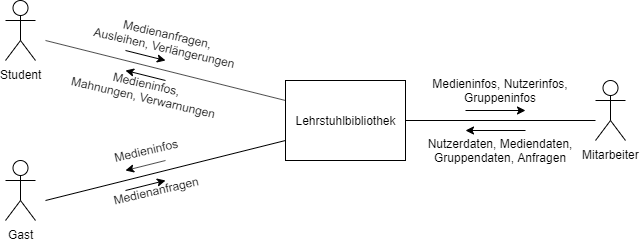
\includegraphics[width=\linewidth]{diagrams/umweltdiagramm.png}
		\caption{Umweltdiagramm}
		\label{fig:umweltdiagramm}
	\end{figure}

\section{Produktfunktionen}
Das Software soll in der Lage sein, die Verwaltung einer Bibliothek durchzuführen. Das heißt, dass
\begin{itemize}
	\item /LF10/ das Ausleihen und Zurückgeben von physischen Medien unterschiedlicher Arten möglich ist
	\item /LF20/ digitale Medien zum Download/Einsicht verfügbar sind
	\item /LF30/ Mahnungen und Rückgabeerinnerungen automatisch versendet werden
	\item /LF40/ Lehrstuhlmitarbeiter eine Übersicht über die aktuell ausgeliehenen Medien erhalten können
	\item /LF50/ das Ausleihen nur Studenten und Mitarbeitern möglich ist
	\item /LF60/ Ausleihen verlängert werden können, wenn das Medium nicht vorbestellt ist
	\item /LF70/ eine Mediensuche über sämtliche Metadaten möglich ist
\end{itemize}

\begin{figure}[h!]
	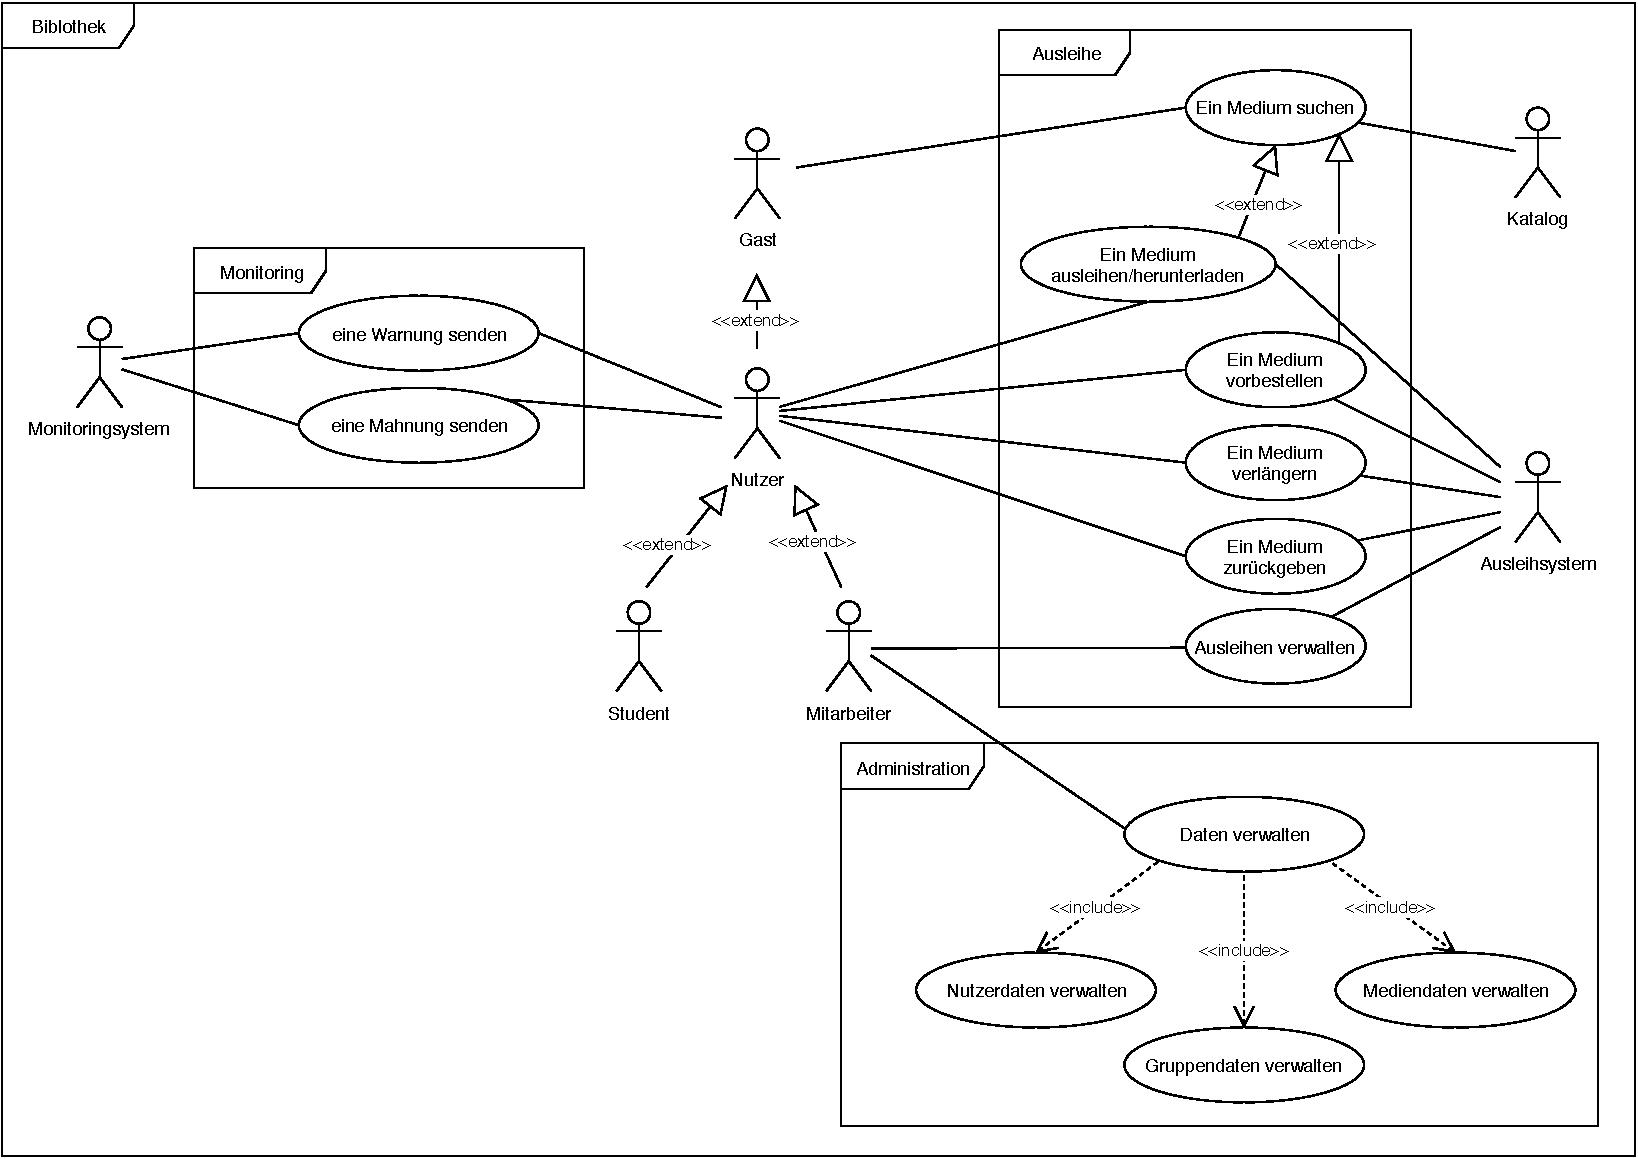
\includegraphics[width=1\linewidth]{diagrams/anwendungsfalldiagramm.pdf} 
	\caption{Anwendungsfalldiagramm von der Bibliothek-System}
	\label{fig:anwendungsfalldiagramm}
\end{figure}

\section{Produktdaten}
\begin{itemize}
	\item /LD10/ die Bibliothek wird auf längere Sicht <50.000 Medien umfassen
\end{itemize}

Die innerhalb eines Jahres voraussichtlich abzuspeichernden Daten sind:
\begin{itemize}
	\item /LD20/ Nutzer- und Gruppeninformationen mit <1.000 Einträgen
	\item /LD30/ Ausleihe- und Monitoringdaten mit <50.000 Einträgen
\end{itemize}

\section{Produktleistungen}
Die Ansprüche an Anfragedauer und Genauigkeit sind:
\begin{itemize}
	\item /LL10/ Anfragezeiten von <2sec für Mediensuchen
	\item /LL20/ Anfragezeiten von <1sec für Nutzer- und Gruppensuchen
	\item /LL30/ Anfragezeiten von <2sec für Ausleihe- und Monitoringdaten
	\item /LL40/ Zeitliche Fristen sind auf 24-Stunden-Basis beschränkt, also reicht eine zeitliche Genauigkeit von 1 min
	\item /LL50/ Abmahngebühren müssen in korrekten Euro-Werten angegeben werden
\end{itemize}

\section{Qualitätsanforderungen}
\newcommand{\xmark}{\ding{55}}%
\begin{table}[h]
	\centering
\begin{tabular}{ || c | c | c | c | c || }
	\hline
	Systemqualität & sehr gut & gut & normal & nicht relevant  \\ \hline
	Funktionalität &  & \xmark &  &  \\ \hline
	Zuverlässigkeit &  & \xmark &  &  \\ \hline
	Benutzbarkeit &  \xmark & &  &  \\ \hline
	Effizienz &  &  & \xmark  &  \\ \hline
	Wartbarkeit &  &  & \xmark &  \\ \hline
	Portabilität &  &  &  & \xmark \\
	\hline
\end{tabular}
\caption{Qualitätszielbestimmung}
\label{table:qualitätsanforderungen}
\end{table}
\begin{itemize}
	\item /LQB10/ Qualitätsanforderung zur Benutzbarkeit des Systems
	\item /LQE10/ Qualitätsanforderung zur Effizienz des Systems
	\item /LQF10/ Qualitätsanforderung zur Funktionalität des Systems
	\item /LQP10/ Qualitätsanforderung zur Portabilität des Systems
	\item /LQW10/ Qualitätsanforderung zur Wartbarkeit des Systems
	\item /LQZ10/ Qualitätsanforderung zur Zuverlässigkeit des Systems
\end{itemize}
\end{document}
